\documentclass[journal]{IEEEtran} % use the `journal` option for ITherm conference style
\IEEEoverridecommandlockouts
% The preceding line is only needed to identify funding in the first footnote. If that is unneeded, please comment it out.
\usepackage{cite}
\usepackage{amsmath,amssymb,amsfonts}
\usepackage{algorithmic}
\usepackage{graphicx}
\usepackage{textcomp}
\usepackage{xcolor}
\usepackage{hyperref}
%\usepackage{algorithm}
\usepackage[ruled, vlined]{algorithm2e}

% Agregar Seudocodigo
\usepackage{listings}
% Paquetes para tigz y agregar el archivo fig.tex
\usepackage{pgfplots}
\pgfplotsset{compat=1.18}
\usepackage{pgfplotstable}
\usepackage{tikz}
\usepackage{caption}

\def\BibTeX{{\rm B\kern-.05em{\sc i\kern-.025em b}\kern-.08em
    T\kern-.1667em\lower.7ex\hbox{E}\kern-.125emX}}
%Agrega nuevo comando para geragr figuras
\newcommand{\misDatos}{(0,0)(1,0)(2,2)(3,0)(4,6)(5,4),(6,7)}
    
\begin{document}

\title{Industrial Communication based on MQTT and
Modbus Communication applied in a
Meteorological Network\\
% delete or comment-out the following line before submission
{\footnotesize \textsuperscript{*}Note: Sub-titles are not captured in Xplore and should not be used}
\thanks{Identify applicable funding agency here. If none, delete this.}
}

\author{%%%% author names
    \IEEEauthorblockN{1\textsuperscript{st} Juan Naula}% first author
    \IEEEauthorblockA{\textit{GIHP4C, Universidad Politecnica Saleciana, Cuenca, Ecuador}}\\% first affiliation
    %%%% corresponding author contact details
    \IEEEauthorblockA{jnaulas@ups.edu.ec}
}

\maketitle

\begin{abstract}
    In this paper, we propose an architecture to enable
hierarchical sensors networks that use MQTT protocol for sensors
data acquisition interact with the MODBUS protocol to send
information to the SCADA system. The proposed architecture
implemented with three stages. In the first stage, we configure
the MQTT protocol in sensors. In the second stage, we configure
the middleware to transport the data to SCADA system by
MODBUS protocol. And in the third stage, the SCADA system
is implemented. We conclude that the architecture proposed is
feasible to hierarchical sensor networks that used the MQTT
protocol and interacts with MODBUS industrial networks.
\end{abstract}

\begin{IEEEkeywords}
    MQTT, modbus, industrial communication,
SCADA.
\end{IEEEkeywords}

\section{Introduction}
The Internet of Things (IoT) will change the way we
live, its technological impact will give intelligence to almost
everything things and will allow the development of cloud
computing since more data can be collected, stored and
analyzed than ever before, as described by authors in \cite{guohuan2009research}.

In this regard, as described in \cite{@inproceedingsdai2004unifying,8789574} the IoT is growing
and is expected that by 2020 there will be more than two
billion devices connected to Internet. In the same way, in
\cite{akyildiz2002wireless}, \cite{alani2014osi,banks2014mqtt,bworldm}, the authors emphasize that interconnected things
uses existing Internet standards to provide information transfer
services, analysis, applications and communications, i.e., not
only collects information from the environment (detection)
to interact with the physical world (action/command/control)
independently.
\section{General System Architecture}
In Fig. \ref{Fig1:1} we showed the General System Architecture above
described.

\begin{figure}[h!]
    \centering
    \includegraphics[width=0.4\textwidth]{Figuras/fig1.pdf}
    \caption{general System Architecture}
    \label{Fig1:1}
\end{figure}

\subsection{Algorithm}
\begin{algorithm}
%Alinea el algoritmo
    \SetAlgoLined
    \KwResult {Write here the result}
    initialization\;
    \While{while condition}{
        instructions\;
        \eIf{condition}{
        instructions 1\;
        instructions  1\;
        }{
        instruction3\;
        }
    }
    \caption{How to write algorithm}
\end{algorithm}

\section{Pseudocode}
%Crear seudo codigo en python
\begin{itemize}
    \item Python

    \begin{lstlisting}[language=Python]
        ## Programa que escriba numetos
        ## impares desde 100 hasta la unidad
        ## y calcule la suma
        n=100
        def mi_funcion(n, acum):
        acum:0
        while n>=1:
        if n%2 !=0:
        print n
        acum +=n
        n-=1
        print 'y su suma es: '+str(acum)
        mu_funcion(n)
    \end{lstlisting}
    \item C
    \begin{lstlisting}[language=c, breaklines=true]
        #include <stdio.h>
        #define N10
        /*
        Comenrario en un bloque
        */
        int main()
        {
        int i;

        //line coment
        puts(hola mundo);
            for(i=0; i<N;i+++)
            {
                puts("\LaTeX es genial para los programadores");
            }
            return 0;
        }
    \end{lstlisting}
\end{itemize}
% Agrega al punto en el que lo generamos [h!]

\section{TIKZ}
\begin{figure}[h!]
    \centering
    % Para dar tama�o a la figura
    \resizebox{.85\linewidth}{!}{

\tikzset{every picture/.style={line width=0.75pt}} %set default line width to 0.75pt        

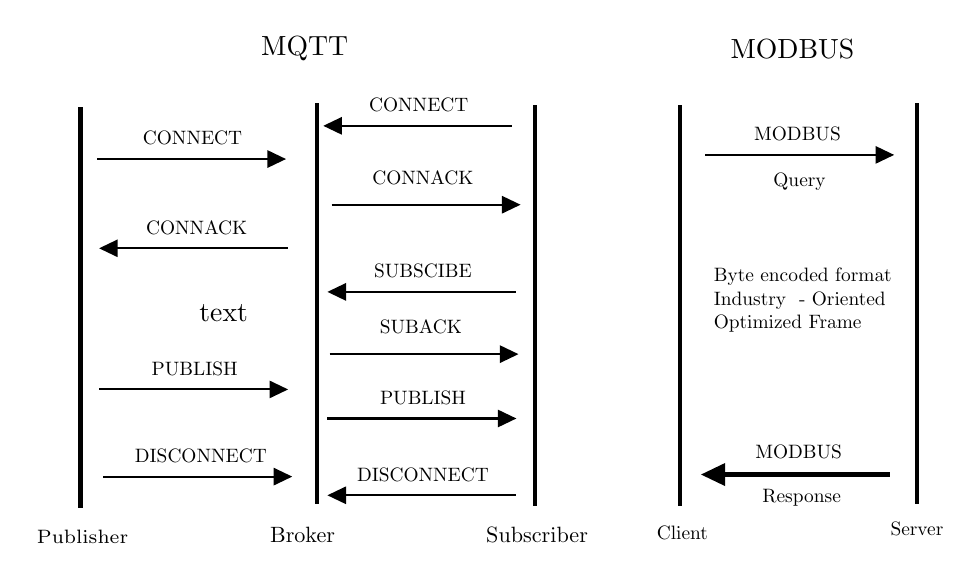
\begin{tikzpicture}[x=0.75pt,y=0.75pt,yscale=-1,xscale=1]
%uncomment if require: \path (0,300); %set diagram left start at 0, and has height of 300

%Straight Lines [id:da12798558333744703] 
\draw [line width=1.5]    (51,51) -- (51,244) ;


%Straight Lines [id:da11517902673265334] 
\draw [line width=1.5]    (165,49) -- (165,242) ;


%Straight Lines [id:da27778345517546654] 
\draw [line width=1.5]    (270,50) -- (270,243) ;


%Straight Lines [id:da4784433104779049] 
\draw [line width=1.5]    (340,50) -- (340,243) ;


%Straight Lines [id:da14318622021376104] 
\draw [line width=1.5]    (454,49) -- (454,242) ;


%Straight Lines [id:da2521307853666861] 
\draw [color={rgb, 255:red, 0; green, 0; blue, 0 }  ,draw opacity=1 ][line width=0.75]    (59,76) -- (148,76) ;
\draw [shift={(150,76)}, rotate = 180] [fill={rgb, 255:red, 0; green, 0; blue, 0 }  ,fill opacity=1 ][line width=0.75]  [draw opacity=0] (8.93,-4.29) -- (0,0) -- (8.93,4.29) -- cycle    ;

%Straight Lines [id:da416495389819703] 
\draw [color={rgb, 255:red, 0; green, 0; blue, 0 }  ,draw opacity=1 ][line width=0.75]    (62,119) -- (151,119) ;

\draw [shift={(60,119)}, rotate = 0] [fill={rgb, 255:red, 0; green, 0; blue, 0 }  ,fill opacity=1 ][line width=0.75]  [draw opacity=0] (8.93,-4.29) -- (0,0) -- (8.93,4.29) -- cycle    ;
%Straight Lines [id:da9635625455331085] 
\draw [color={rgb, 255:red, 0; green, 0; blue, 0 }  ,draw opacity=1 ][line width=0.75]    (60,187) -- (149,187) ;
\draw [shift={(151,187)}, rotate = 180] [fill={rgb, 255:red, 0; green, 0; blue, 0 }  ,fill opacity=1 ][line width=0.75]  [draw opacity=0] (8.93,-4.29) -- (0,0) -- (8.93,4.29) -- cycle    ;

%Straight Lines [id:da1895725774033723] 
\draw [color={rgb, 255:red, 0; green, 0; blue, 0 }  ,draw opacity=1 ][line width=0.75]    (62,229) -- (151,229) ;
\draw [shift={(153,229)}, rotate = 180] [fill={rgb, 255:red, 0; green, 0; blue, 0 }  ,fill opacity=1 ][line width=0.75]  [draw opacity=0] (8.93,-4.29) -- (0,0) -- (8.93,4.29) -- cycle    ;

%Straight Lines [id:da7272521685262943] 
\draw [color={rgb, 255:red, 0; green, 0; blue, 0 }  ,draw opacity=1 ][line width=0.75]    (170,60) -- (259,60) ;

\draw [shift={(168,60)}, rotate = 0] [fill={rgb, 255:red, 0; green, 0; blue, 0 }  ,fill opacity=1 ][line width=0.75]  [draw opacity=0] (8.93,-4.29) -- (0,0) -- (8.93,4.29) -- cycle    ;
%Straight Lines [id:da30340216601848824] 
\draw [color={rgb, 255:red, 0; green, 0; blue, 0 }  ,draw opacity=1 ][line width=0.75]    (172,98) -- (261,98) ;
\draw [shift={(263,98)}, rotate = 180] [fill={rgb, 255:red, 0; green, 0; blue, 0 }  ,fill opacity=1 ][line width=0.75]  [draw opacity=0] (8.93,-4.29) -- (0,0) -- (8.93,4.29) -- cycle    ;

%Straight Lines [id:da5689262114397526] 
\draw [color={rgb, 255:red, 0; green, 0; blue, 0 }  ,draw opacity=1 ][line width=0.75]    (172,140) -- (261,140) ;

\draw [shift={(170,140)}, rotate = 0] [fill={rgb, 255:red, 0; green, 0; blue, 0 }  ,fill opacity=1 ][line width=0.75]  [draw opacity=0] (8.93,-4.29) -- (0,0) -- (8.93,4.29) -- cycle    ;
%Straight Lines [id:da43739445383533293] 
\draw [color={rgb, 255:red, 0; green, 0; blue, 0 }  ,draw opacity=1 ][line width=0.75]    (171,170) -- (260,170) ;
\draw [shift={(262,170)}, rotate = 180] [fill={rgb, 255:red, 0; green, 0; blue, 0 }  ,fill opacity=1 ][line width=0.75]  [draw opacity=0] (8.93,-4.29) -- (0,0) -- (8.93,4.29) -- cycle    ;

%Straight Lines [id:da4265213474229044] 
\draw [color={rgb, 255:red, 0; green, 0; blue, 0 }  ,draw opacity=1 ][line width=0.75]    (170,201) -- (259,201) ;
\draw [shift={(261,201)}, rotate = 180] [fill={rgb, 255:red, 0; green, 0; blue, 0 }  ,fill opacity=1 ][line width=0.75]  [draw opacity=0] (8.93,-4.29) -- (0,0) -- (8.93,4.29) -- cycle    ;

%Straight Lines [id:da2890367081898375] 
\draw [color={rgb, 255:red, 0; green, 0; blue, 0 }  ,draw opacity=1 ][line width=0.75]    (172,238) -- (261,238) ;

\draw [shift={(170,238)}, rotate = 0] [fill={rgb, 255:red, 0; green, 0; blue, 0 }  ,fill opacity=1 ][line width=0.75]  [draw opacity=0] (8.93,-4.29) -- (0,0) -- (8.93,4.29) -- cycle    ;
%Straight Lines [id:da5478425871587402] 
\draw [color={rgb, 255:red, 0; green, 0; blue, 0 }  ,draw opacity=1 ][line width=0.75]    (352,74) -- (441,74) ;
\draw [shift={(443,74)}, rotate = 180] [fill={rgb, 255:red, 0; green, 0; blue, 0 }  ,fill opacity=1 ][line width=0.75]  [draw opacity=0] (8.93,-4.29) -- (0,0) -- (8.93,4.29) -- cycle    ;

%Straight Lines [id:da6706223138763108] 
\draw [color={rgb, 255:red, 0; green, 0; blue, 0 }  ,draw opacity=1 ][line width=1.5]    (353,228) -- (441,228) ;

\draw [shift={(350,228)}, rotate = 0] [fill={rgb, 255:red, 0; green, 0; blue, 0 }  ,fill opacity=1 ][line width=1.5]  [draw opacity=0] (11.61,-5.58) -- (0,0) -- (11.61,5.58) -- cycle    ;

% Text Node
\draw (159,23) node  [align=left] {MQTT};
% Text Node
\draw (394,23) node  [align=left] {MODBUS};
% Text Node
\draw (52,258) node  [align=left] {{\scriptsize Publisher}};
% Text Node
\draw (158,257) node [scale=0.8] [align=left] {Broker};
% Text Node
\draw (271,257) node [scale=0.8] [align=left] {Subscriber};
% Text Node
\draw (105,66) node [scale=0.7] [align=left] {CONNECT};
% Text Node
\draw (107,109) node [scale=0.7] [align=left] {CONNACK};
% Text Node
\draw (106,177) node [scale=0.7] [align=left] {PUBLISH};
% Text Node
\draw (109,219) node [scale=0.7] [align=left] {DISCONNECT};
% Text Node
\draw (214,50) node [scale=0.7] [align=left] {CONNECT};
% Text Node
\draw (216,85) node [scale=0.7] [align=left] {CONNACK};
% Text Node
\draw (216,130) node [scale=0.7] [align=left] {SUBSCIBE};
% Text Node
\draw (215,157) node [scale=0.7] [align=left] {SUBACK};
% Text Node
\draw (216,191) node [scale=0.7] [align=left] {PUBLISH};
% Text Node
\draw (216,228) node [scale=0.7] [align=left] {DISCONNECT};
% Text Node
\draw (398,64) node [scale=0.7] [align=left] {MODBUS };
% Text Node
\draw (399,87) node [scale=0.7] [align=left] {Query };
% Text Node
\draw (397,217) node [scale=0.7] [align=left] {MODBUS};
% Text Node
\draw (400,239) node [scale=0.7] [align=left] {Response };
% Text Node
\draw (341,256) node [scale=0.7] [align=left] {Client};
% Text Node
\draw (454,254) node [scale=0.7] [align=left] {Server};
% Text Node
\draw (399,144) node [scale=0.7] [align=left] {Byte encoded format\\Industry \ - Oriented \\Optimized Frame};
% Text Node
\draw (120,150) node  [align=left] {text};


\end{tikzpicture}}
    \caption{Caption}
    \label{fig:enter-label}
\end{figure}

\begin{center}
    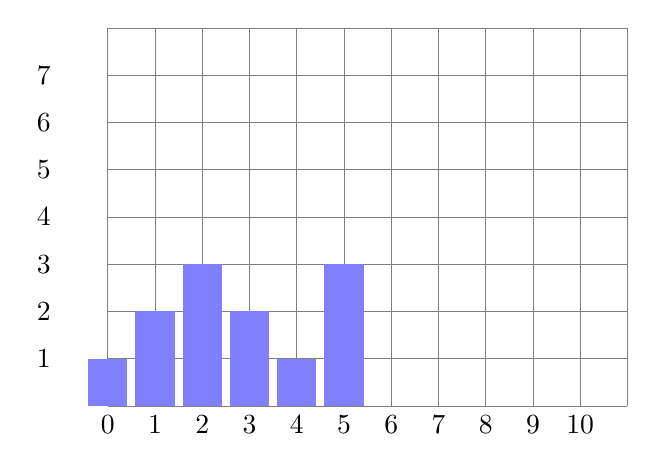
\begin{tikzpicture}[scale=0.6] 
        \draw[very thin, gray] (0,0) grid(11,8);
        \foreach \y in{1,2,...,7} \draw(-1,\y)node[left]{\y};
        \foreach \x in{0,1,...,10} \draw(\x,0)node[below]{\x};
        \def\misDatos{(0,1) (1,2) (2,3) (3,2) (4,1) (5,3)}
        \draw[line width=5mm,color=blue!50] plot[ycomb] coordinates{\misDatos};
    \end{tikzpicture}
    \captionof{figure}{\text{Confusion matrix}}
    \label{BARRA}
\end{center}

\section*{Acknowledgment}



\section*{References}

\bibliographystyle{IEEEtran}
\bibliography{bibl.bib}


\end{document}
